\documentclass{article}
\usepackage[utf8]{inputenc}
\usepackage{geometry}
 \geometry{
 a4paper,
 total={170mm,257mm},
 left=20mm,
 top=20mm,
 }
 \usepackage{graphicx}
 \usepackage{titling}

\title{\textbf{Assignment 1:} Fast Trajectory Replanning}
\author{Ehsan, Goldstein}
\date{February 2023}
 
 \usepackage{fancyhdr}
\fancypagestyle{plain}{%  the preset of fancyhdr 
    \fancyhf{} % clear all header and footer fields
    \fancyfoot[C]{\thepage}
    \fancyhead[L]{CS440 Intro to AI}
    \fancyhead[R]{\theauthor}
}
\makeatletter
\def\@maketitle{%
  \newpage
  \null
  \vskip 1em%
  \begin{center}%
  \let \footnote \thanks
    {\LARGE \@title \par}%
    \vskip 1em%
    %{\large \@date}%
  \end{center}%
  \par
  \vskip 1em}
\makeatother

\usepackage{lipsum}  
\usepackage{cmbright}

\begin{document}

\maketitle

\noindent\begin{tabular}{@{}ll}
    \textbf{Submitted By: }Brandon Goldstein (bbg17), Taqiya Ehsan (te137)\\
     \textbf{Date: } 21 February 2023
\end{tabular}

\subsection*{Part 0}
The \texttt{CS 440 Assignment Final} file contains an algorithm, \texttt{generate\(\_\)mazes()}, to generate 50 101x101 mazes. Each maze is initiated as a numpy array of all zeros. A  point is then chosen at random as the starting point for the depth first search (DFS) algorithm. A cell when visited is marked blocked with a 30 percent probability. The DFS algorithm runs as long as all the cells have not been visited and marked blocked (0) or unblocked (1) with 30-70 odds. A sample maze has been illustrated in Figure 1, where blue indicates a blocked cell and yellow indicates an unblocked cell:

\begin{figure}[!htbp]
\centering
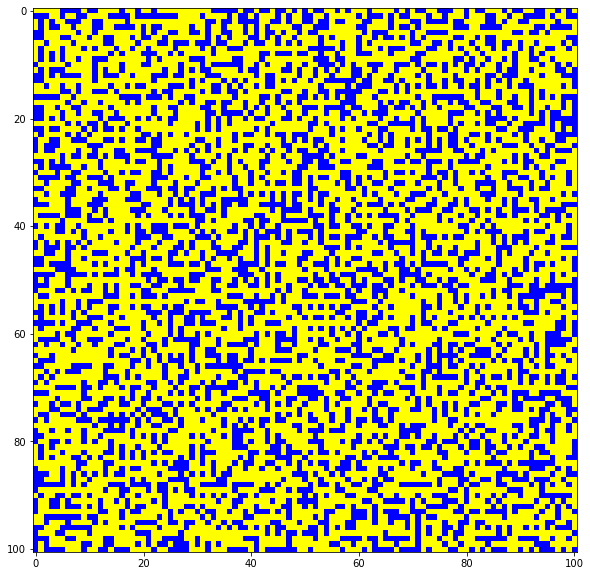
\includegraphics[width=0.5\textwidth, height=0.5\textheight,keepaspectratio]{maze_big.png}
\caption{Sample Maze}
    \label{fig:Map}
\end{figure}

\noindent
All 50 mazes are generated similarly, with random starting points for the DFS algorithm. All mazes can be stored as \texttt{txt}files and loaded as numpy arrays of 0s and 1s. The grid in Figure 2 visualizes all the mazes for a particular call of \texttt{generate\(\_\)mazes()}.\\

\begin{figure}[!htbp]
\centering
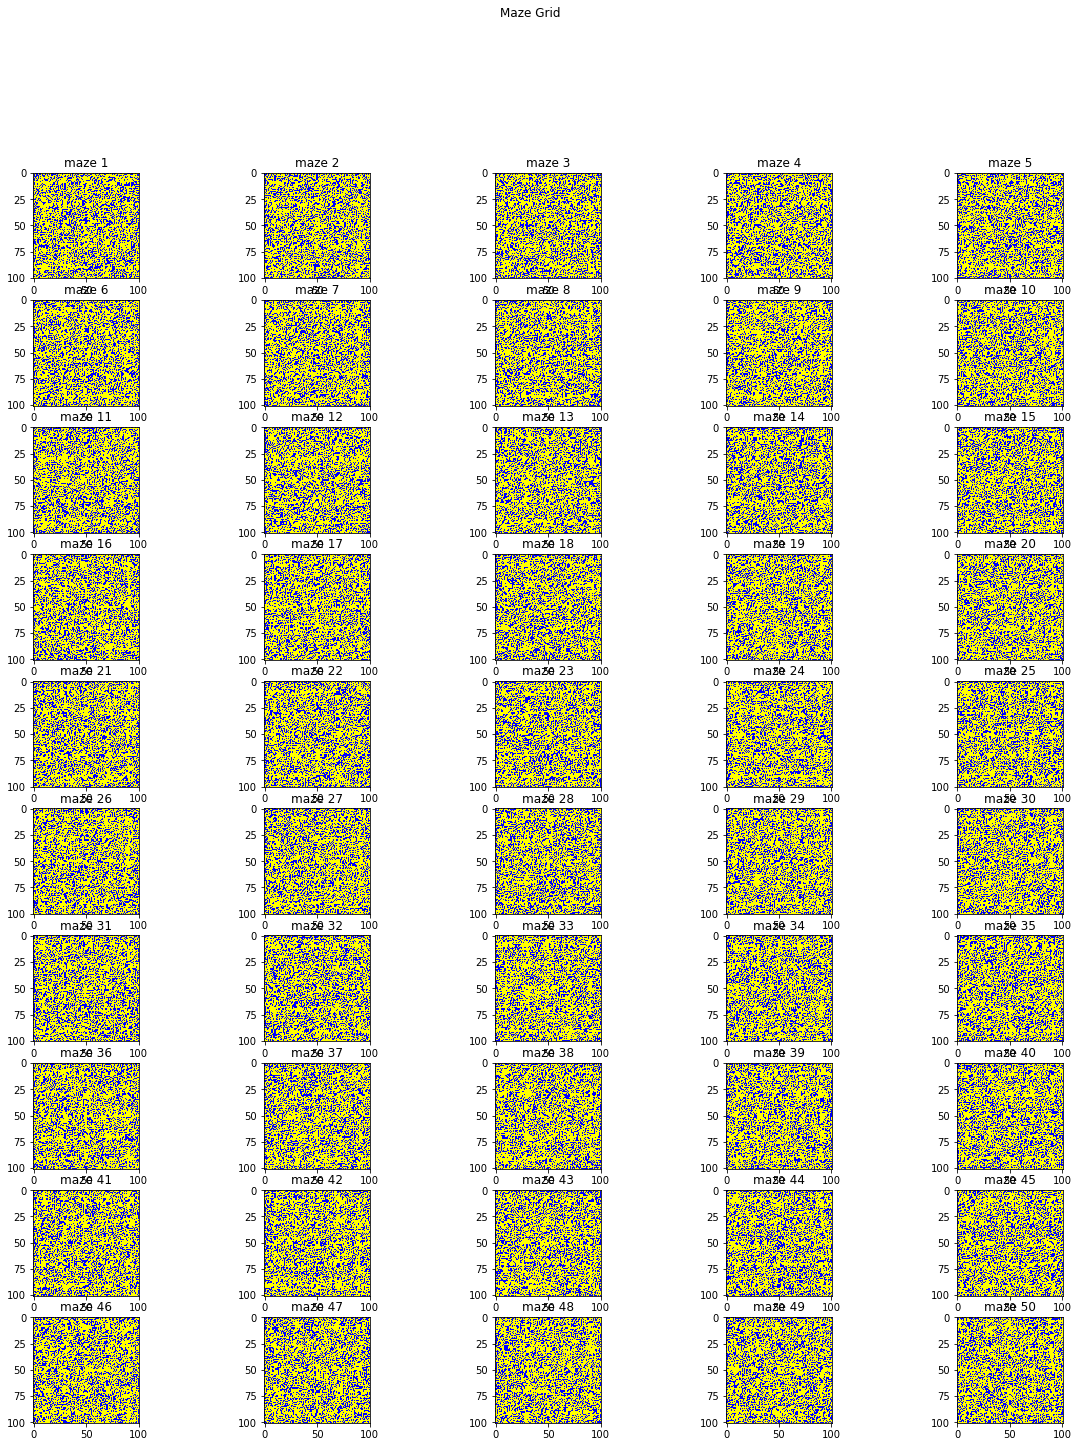
\includegraphics[width=0.5\textwidth, height=0.5\textheight,keepaspectratio]{maze_grid.png}
\caption{Maze Grid}
    \label{fig:Map}
\end{figure}

\noindent
To annotate the path determined by the A* algorithm, we change the entries of the coordinates included within the path from 1 to 2 and map the value 2 to red. Figure 3 is a sample of the most optimal path from start location (0, 0) to goal location (20, 20) on the sample maze in Figure 1.

\begin{figure}[!htbp]
\centering
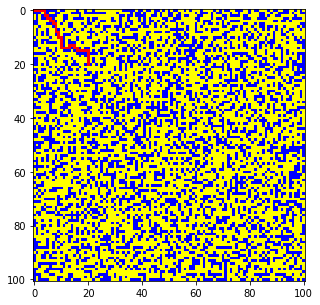
\includegraphics[width=0.5\textwidth, height=0.5\textheight,keepaspectratio]{maze_with_path.png}
\caption{Maze with Path}
    \label{fig:Map}
\end{figure}

\subsection*{Part 1}
\subsubsection*{a} In Figure 8 of the assignment write-up, the agent starts at cell E2. From this location, it can go in one of 3 directions – north, east, or west (south is a dead end). The objective of the agent is to reach the target cell along the path with the least cost function value. If the agent moves east, it can reach the target in only 3 moves, not taking the blocked cells into account. On the other hand, moving north or west would require more moves, or a higher cost, to reach the target. That is why the agent, who does not know about the blocked cells yet, moves east first, as that is seemingly the path to the target with the lowest cost.

\subsubsection*{b} Since the gridworld is finite, there is a finite number of paths that are of a finite length that the agent can follow to reach the target. We know that the paths must be of finite length because an infinite length would imply the existence of cycles; cycles are not allowed by A*. These paths will either successfully take the agent to the target or will demonstrate the impossibility of reaching the target because of blocked cells. As there are a finite number of paths and they are of finite length, the agent can either reach the target or discovers that this is impossible in finite time by iterating over the paths. Note, the agent will only stop moving along a selected path if it reaches the target or discovers that the path is blocked. Once the agent has discovered barriers around a cell, the agent remembers them and will not build a path into them again. Thus, the agent will not stop in the same cell more than once. Consequently, the agent will build and move along a path starting at a given unblocked cell at most once, so it builds at most n paths on which it can immediately move (where n is the number of unblocked cells). These paths contain, at most, every unblocked cell once. If a path contained an unblocked cell more than once, it would not be the shortest path from the agent to the target (which A* does not allow) because it would contain a cycle. So, the agent can move through a maximum of n paths of maximum length n. Consequently, the number of moves of the agent until it reaches the target or discovers that doing so is impossible is bounded from above by the number of unblocked cells squared.  

\subsection*{Part 2}
We implemented both versions of Repeated Forward A* and executed them on 50 101x101 gridworlds with start state (0,0) and goal state (20,20). These gridworlds were selected by generating gridworlds (the process for which is detailed in Part 0) and assessing the existence of a viable path from (0,0) to (20,20). If such a path existed, the gridworld was saved. Gridworlds were saved until 50 were collected. The table below (Table 1) shows the mean number of expanded cells and the standard deviation for the executions of the two versions of Repeated Forward A* on the 50 gridworlds. The version of Repeated Forward A* which breaks ties in favor of cells with larger g-values performed significantly better on-average than the version of Repeated Forward A* which breaks ties in favor of cells with smaller g-values, as shown by the means in Table 1. Moreover, the version of Repeated Forward A* which breaks ties in favor of cells with larger g-values expanded fewer cells for every gridworld. The performance of the version of Repeated Forward A* which breaks ties in favor of cells with larger g-values is also notably more consistent than the version of Repeated Forward A* which breaks ties in favor of cells with smaller g-values, as shown by the standard deviations in Table 1. The differences in performance are due to the implications of tie-breaking in favor of larger or smaller g-values. As we move toward the goal state, the g-values increase and the h-values decrease. So, if we break ties in favor of larger g-values, Repeated Forward A* prefers to expand cells close to the goal state. If we break ties in favor of smaller g-values, Repeated Forward A* prefers to expand cells close to the start state. In other words, breaking ties in favor of larger g-values results in Repeated Forward A* exploring the gridworld less (which entails expanding fewer cells) and attempting to rush to the goal state. Of course, this implies that breaking ties in favor of smaller g-values results in Repeated Forward A* exploring the gridworld more (which entails expanding more cells), hence the results detailed above and in Table 1.\\ 

\begin{table}[!h]
    \centering
    \small
    \begin{tabular}{cccc}
        \hline
         Variant & Mean Expanded Cells & Standard Deviation\\
         \hline
         Larger g-values & 762.04 & 653.66\\
         Smaller g-values & 3468.82 & 1386.44\\
        \hline
    \end{tabular}
    \caption{The Effects of Ties}
    \label{tab:my_label}
\end{table}

\subsection*{Part 3}
We implemented Repeated Forward A* and Repeated Backward A* and executed them on 50 101x101 gridworlds with start state (0,0) and goal state (20,20). These are the same gridworlds from Part 2. As shown in Table 2, Repeated Forward A* boasts a lower mean number of expanded cells than Repeated Backward A* and more consistent performance, with a lower standard deviation than Repeated Backward A*. Notably, Repeated Backward A* expanded fewer cells, when compared to Repeated Forward A*, for 24 of the 50 (48 percent) gridworlds. The difference in performance between Repeated Forward A* and Repeated Backward A* is the result of the gridworld design. As both Repeated Forward A* and Repeated Backward A* employ a heuristic that prioritizes expanding cells closest to the goal state and breaking ties in favor of cells closer to the goal state, they will be impacted by the location of obstacles relative to the start and goal states. Gridworlds that have more obstacles around the start state benefit Repeated Backward A*, as Repeated Forward A* will run into obstacles early, call its internal A*, and expand cells from an area approximate to the start state towards its goal state. Repeated Backward A* will discover these obstacles as well, but it will do so when it is already close to the start state (the goal state of Repeated Backward A*). As Repeated Backward A* is closer to its goal state when it calls its internal A*, it will expand fewer cells than Repeated Forward A* when making a new path. Gridworlds that have more obstacles around the goal state benefit Repeated Forward A* by similar logic. So, for this set of gridworlds, it is reasonable to conjecture that there might be a greater distribution of obstacles around (20,20) than (0,0).\\

\begin{table}[!h]
    \centering
    \small
    \begin{tabular}{cccc}
        \hline
         Variant & Mean Expanded Cells & Standard Deviation\\
         \hline
         Forward & 762.04 & 653.66\\
         Backward & 965.02 & 913.28\\
        \hline
    \end{tabular}
    \caption{Forward vs Backward}
    \label{tab:my_label}
\end{table}

\subsection*{Part 4}
To start, h-values \textit{h(s)} are consistent if and only if they satisfy the triangle inequalities $h(s_{goal}) = 0$ and $h(s) \leq c(s,a) + h(succ(s,a))$ for all states \textit{s} with $s \neq s_{goal}$ and all actions \textit{a} that can be executed in state \textit{s}. By definition, when \textit{h(s)} is the Manhattan distance, $h(s) = |x(s)-x(s_{goal})| + |y(s)-y(s_{goal})|$, where $x(s)$ is the x-coordinate of state \textit{s} in the gridworld and $y(s)$ is the y-coordinate of state \textit{s} in the gridworld. Consequently, $h(s_{goal}) = |x(s_{goal})-x(s_{goal})| + |y(s_{goal})-y(s_{goal})| = 0$. For arbitrary state \textit{s} with $s \neq s_{goal}$ and arbitrary action \textit{a} that can be executed in state \textit{s}, $h(s) = |x(s)-x(s_{goal})| + |y(s)-y(s_{goal})| = |x(s)-x(s_{goal})+x(succ(s,a))-x(succ(s,a))| + |y(s)-y(s_{goal})+y(succ(s,a))-y(succ(s,a))|$. By the triangle inequality, $|x(s)-x(s_{goal})+x(succ(s,a))-x(succ(s,a))| + |y(s)-y(s_{goal})+y(succ(s,a))-y(succ(s,a))| \leq |x(s)-x(succ(s,a))| + |x(succ(s,a))-x(s_{goal})| + |y(s)-y(succ(s,a))| + |y(succ(s,a))-y(s_{goal})| = |x(s)-x(succ(s,a))| + |y(s)-y(succ(s,a))| + h(succ(s,a))$. If the agent exists in a gridworld in which the agent can move only in the four main compass directions, by construction, $|x(s)-x(succ(s,a))| + |y(s)-y(succ(s,a))| \leq c(s,a)$. So, $|x(s)-x(succ(s,a))| + |y(s)-y(succ(s,a))| + h(succ(s,a)) \leq c(s,a) + h(succ(s,a))$. Thus, $h(s) \leq c(s,a) + h(succ(s,a))$. So, Manhattan distances are consistent in gridworlds in which the agent can move only in the four main compass directions.     
\newline
\newline
\noindent
From above, we know that the initial h-values are consistent. Assume that action costs can increase. Let $c(s,a)$ denote initial action costs and $c^{'}(s,a)$ denote increased action costs. By definition, $c(s,a) \leq c^{'}(s,a)$, which implies that $c(s,a) + h(succ(s,a)) \leq c^{'}(s,a) + h(succ(s,a))$ for all states \textit{s} with $s \neq s_{goal}$ and all actions \textit{a} that can be executed in state \textit{s}. We must consider three cases to prove that Adaptive A* leaves initially consistent h-values consistent even if action costs can increase. Consider arbitrary state \textit{s} with $s \neq s_{goal}$ and arbitrary action \textit{a} that can be executed in state \textit{s}. For case 1, assume \textit{s} and $succ(s,a)$ are expanded. As \textit{s} and $succ(s,a)$ are expanded, $h_{new}(s) = g(s_{goal}) - g(s)$ and $h_{new}(succ(s,a)) = g(succ(s,a)_{goal}) - g(succ(s,a))$. Note, $g(s_{goal}) = g(succ(s,a)_{goal})$ by definition. As \textit{s} is expanded, there exists a path from \textit{s} to $succ(s,a)$ with cost $c(s,a) + g(s)$. Accordingly, $g(succ(s,a)) \leq c(s,a) + g(s)$. So, $h_{new}(s) = g(s_{goal}) - g(s) \leq g(s_{goal}) - g(succ(s,a)) + c(s,a) = h_{new}(succ(s,a)) + c(s,a)$. For case 2, assume only \textit{s} is expanded. As only \textit{s} is expanded, $h_{new}(s) = g(s_{goal}) - g(s)$ and $h_{new}(succ(s,a)) = h(succ(s,a))$. Again, as \textit{s} is expanded, there exists a path from \textit{s} to $succ(s,a)$ with cost $c(s,a) + g(s)$. Hence, $g(succ(s,a)) \leq c(s,a) + g(s)$. As $succ(s,a)$ is not expanded, $g(s_{goal}) \leq f(succ(s,a))$. Altogether, $h_{new}(s) = g(s_{goal}) - g(s) \leq f(succ(s,a)) - g(s) = h(succ(s,a)) + g(succ(s,a)) - g(s) = h_{new}(succ(s,a)) + g(succ(s,a)) - g(s) \leq h_{new}(succ(s,a)) + g(succ(s,a)) - g(succ(s,a)) + c(s,a) = h_{new}(succ(s,a)) + c(s,a)$. For case 3, assume \textit{s} is not expanded. Because \textit{s} is not expanded, $h_{new}(s) = h(s)$. It was shown in the assignment write-up that $h(succ(s,a)) \leq h_{new}(succ(s,a))$. As the initial h-values are consistent, $h_{new}(s) = h(s) \leq h(succ(s,a)) + c(s,a) \leq h_{new}(succ(s,a)) + c(s,a)$. To conclude the proof, we must only additionally show that $h_{new}(s_{goal}) = 0$. As the initial h-values are consistent, $h(s_{goal}) = 0$. As the goal state is never expanded, $h_{new}(s_{goal}) = h(s_{goal}) = 0$. So, Adaptive A* leaves initially consistent h-values consistent even if action costs can increase.
\newline
\newline
\noindent
The proof that Adaptive A* leaves initially consistent h-values consistent even if action costs can increase is based on Koenig, S., and Likhachev, M. (2006). A New Principle for Incremental Heuristic Search: Theoretical Results. \textit{International Conference on Automated Planning and Scheduling}. This resource was cited in the assignment write-up. 

\subsection*{Part 5}
We implemented Repeated Forward A* and Adaptive A* and executed them on 50 101x101 gridworlds with start state (0,0) and goal state (20,20). These are the same gridworlds from Part 2. As expected, the mean runtime is lower for Adaptive A*, as see in in Table 3, which suggests better on-average performance from Adaptive A*. This better on-average performance is in spite of the additional bookkeeping done by Adaptive A* (updating the h-values of cells expanded in calls of its internal A*). On a girdworld-level basis, Repeated Forward A* has a lower runtime for 30 of the 50 (60 percent) gridworlds. Relatedly, Adaptive A* expands fewer cells on average, as seen in Table 4, but Repeated Forward A* expands fewer cells for 24 of the 50 (48 percent) gridworlds. The conflict between Adaptive A*'s lower mean number of expansions and the almost even split among gridworlds is not surprising given the relative closeness of the means and the standard deviations of the two variants. In total, the results are mixed, with no clear domination from either algorithm but a distinct edge for Adaptive A*. This edge is derived from Adaptive A*'s construction. Adaptive A* updates the h-values of cells that were expanded in previous calls of its internal A*. As a result, successor calls of the internal A* are more focused, a consequence of which is the faster production of a path from the start state to the goal state. Outcomes in which Repeated Forward A* performed fewer expansions may stem from the random element of the priority queue tiebreaker or the method in which the gridworlds were designed (which places obstacles at random with fixed probabilities).\\

\begin{table}[!h]
    \centering
    \small
    \begin{tabular}{cccc}
        \hline
         Variant & Mean Runtime & Standard Deviation\\
         \hline
         Repeated & 1.59 x 10^{-2} & 1.13 x 10^{-2}\\
         Adaptive & 1.53 x 10^{-2} & 8.46 x 10^{-3}\\
        \hline
    \end{tabular}
    \caption{Heuristics in the Adaptive A* (Runtime)}
    \label{tab:my_label}
\end{table}

\begin{table}[!h]
    \centering
    \small
    \begin{tabular}{cccc}
        \hline
         Variant & Mean Expanded Cells & Standard Deviation\\
         \hline
         Repeated & 762.04 & 653.66\\
         Adaptive & 661.92 & 406.69\\
        \hline
    \end{tabular}
    \caption{Heuristics in the Adaptive A* (Cell Expansions)}
    \label{tab:my_label}
\end{table}

\subsection*{Part 6}
Consider Part 3 in the assignment write-up. It asks us to compare the performance differences between Repeated Forward A* and Repeated Backward A*. We can use a statistical hypothesis test to determine whether such differences are systemic in nature. We can perform a statistical hypothesis test, namely a two-sample paired z-test, by adhering to the following procedure. First, select at least 30 gridworlds at random for which there exists a path from (0,0) to (100, 100) in the gridworld. These gridworlds are the sample. From there, for each gridworld in the sample, execute Repeated Forward A* and Repeated Backward A* with start state (0,0) and goal state (100,100). Document the difference between the number of cells expanded by Repeated Forward A* and the number of cells expanded by Repeated Backward A* for each gridworld. With these differences, we may calculate the sample mean difference in the number of cells expanded by Repeated Forward A* and the number of cells expanded by Repeated Backward A* and the sample standard deviation of the differences in the number of cells expanded by Repeated Forward A* and the number of cells expanded by Repeated Backward A*. With the sample mean difference and sample standard deviation of the differences in hand, we should declare our null hypothesis and alternate hypothesis. Our null hypothesis is that the population mean difference is equal to 0. Our alternate hypothesis is that the population mean difference is not equal to 0. Next, we will calculate the test statistic for our statistical hypothesis test, the two-sample paired z-test. As there are at least 30 gridworlds in our sample, by the Central Limit Theorem, the test statistic $z = \bar{d}/(s_{d}/\sqrt{n})$, where $\bar{d}$ is the sample mean difference, $s_{d}$ is the sample standard deviation of the differences, and $n$ is the number of gridworlds in the sample. Note, because of the nature of the alternate hypothesis, this two-sample paired z-test is a two-tailed statistical hypothesis test. We now set a significance level $\alpha$. With $\alpha$, we find the corresponding z-statistic for a two-tailed statistical hypothesis test, $z_{1-\alpha/2}$. If $\bar{d}<0$ and $z<-z_{1-\alpha/2}$ or if $\bar{d}>0$ and $z>z_{1-\alpha/2}$, we reject the null hypothesis that the population mean difference is equal to 0. If we reject the null hypothesis and $\bar{d}<0$, Repeated Forward A* performs systemically better than Repeated Backward A*. If we reject the null hypothesis and $\bar{d}>0$, Repeated Backward A* performs systemically better than Repeated Forward A*. If we do not reject the null hypothesis, we conclude that the performance differences between Repeated Forward A* and Repeated Backward A* are not systemic in nature.           


\end{document}